\documentclass[11pt]{article}
\usepackage[margin=1in]{geometry}
\usepackage{amsmath,amssymb,amsthm}
\usepackage{graphicx}
\usepackage[hidelinks]{hyperref}

\newtheorem{theorem}{Theorem}
\newtheorem{lemma}{Lemma}
\newtheorem{remark}{Remark}

\newcommand{\A}{A}
\newcommand{\B}{B}
\newcommand{\C}{\mathbb{C}}
\newcommand{\G}{\Gamma}
\newcommand{\K}{K}
\newcommand{\HH}{\mathcal{H}}
\newcommand{\VN}{VN}
\newcommand{\rt}{\rtimes}

\title{A Bernoulli Wreath Product Subcase of the Crann--Tanko QSIN Conjecture}
\author{fa\_banach\_001, agent\_lane\_03}
\date{2026-07-03}

\begin{document}
\maketitle

\section*{Status}

This is a partial result packet for arXiv:1602.05259, Jason Crann and
Zsolt Tanko, \emph{On the operator homology of the Fourier algebra and
its cb-multiplier completion}. The source conjectures that relative
operator \(1\)-biflatness of \(\A(G)\) is equivalent to \(G\) being QSIN.
The theorem below proves the conjecture for compact Bernoulli wreath
products \(K_0^\Gamma\rtimes\Gamma\).

\section*{Source Problem}

The source paper proves that \(\A(G)\) is relatively \(1\)-biflat if and
only if the diagonal \(G_\Delta\) has a contractive approximate indicator
in \(\B(G\times G)\), and then asks whether this is equivalent to QSIN.
The relevant source crop is:

\begin{center}

\includegraphics[width=0.92\linewidth]{figures/open_problem_crop.png}
\end{center}

The source also proves the following semidirect-product obstruction,
which is the main input used here:

\begin{center}
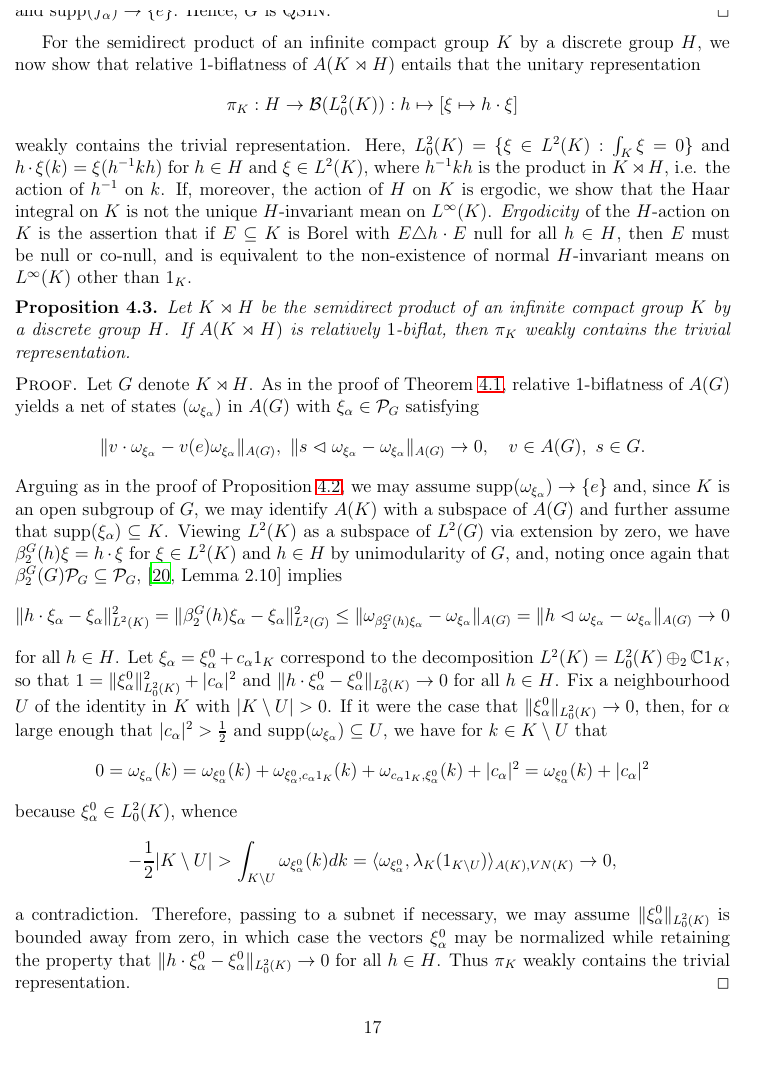
\includegraphics[width=0.78\linewidth]{figures/semidirect_obstruction_crop.png}
\end{center}

\section*{The Result}

Let \(K_0\) be a nontrivial compact group with normalized Haar probability
measure, and let \(\Gamma\) be a discrete group. Put
\[
  K=K_0^\Gamma
\]
with product Haar measure, and let \(\Gamma\) act on \(K\) by the
Bernoulli shift:
\[
  (h\cdot x)_g=x_{h^{-1}g}\qquad(h,g\in\Gamma,\ x\in K).
\]
Form the locally compact semidirect product \(G=K\rtimes\Gamma\).

\begin{theorem}
For \(G=K_0^\Gamma\rtimes\Gamma\) as above, \(\A(G)\) is relatively
\(1\)-biflat if and only if \(\Gamma\) is amenable.
\end{theorem}

\section*{Proof Intuition}

Crann--Tanko show that relative \(1\)-biflatness forces almost invariant
vectors in the Koopman representation of the acting group on
\(L^2_0(K)\). For a Bernoulli compact shift, \(L^2_0(K)\) has a rigid
finite-coordinate decomposition. Each finite-coordinate layer is induced
from the stabilizer of a finite nonempty subset of \(\Gamma\), and that
stabilizer is finite. Hence the whole Koopman representation is weakly
contained in the left regular representation. If it also weakly contains
the trivial representation, then the trivial representation is weakly
contained in the left regular representation, which is exactly amenability
of \(\Gamma\).

\section*{Proof}

We first record the Koopman-representation fact used in the theorem.

\begin{lemma}
Let \(K=K_0^\Gamma\) be a nontrivial compact Bernoulli shift over a
discrete group \(\Gamma\). Let \(\pi_K\) be the unitary representation of
\(\Gamma\) on \(L^2_0(K)\) induced by the shift action. Then
\[
  \pi_K \prec \lambda_\Gamma,
\]
where \(\lambda_\Gamma\) is the left regular representation and
\(\prec\) denotes weak containment.
\end{lemma}

\begin{proof}
Write
\[
  L^2(K_0)=\C 1\oplus H_0
\]
with \(H_0=L^2_0(K_0)\). Since \(K_0\) is nontrivial, \(H_0\neq 0\).
The finite-coordinate cylinder functions give the Hilbert direct sum
decomposition
\[
  L^2_0(K_0^\Gamma)
  =
  \bigoplus_{\varnothing\neq F\subseteq\Gamma,\ F\text{ finite}}
  H_F,
  \qquad
  H_F=\bigotimes_{g\in F} H_0,
\]
where all coordinates outside \(F\) are constants. The Bernoulli shift
sends \(H_F\) onto \(H_{hF}\).

Fix a finite nonempty subset \(F\subseteq\Gamma\), and let
\(\Gamma_F=\{h\in\Gamma:hF=F\}\). The left translation action of
\(\Gamma_F\) on \(F\) is faithful: if \(hf=f\) for one \(f\in F\), then
\(h=e\). Thus \(\Gamma_F\) embeds into the finite permutation group of
\(F\), and is finite. The summand generated by the orbit of \(H_F\) is
unitarily equivalent to an induced representation
\[
  \operatorname{Ind}_{\Gamma_F}^{\Gamma}(\sigma_F),
\]
where \(\sigma_F\) is the natural unitary representation of the finite
group \(\Gamma_F\) on \(H_F\).

Because \(\Gamma_F\) is finite, it is amenable, and every unitary
representation of \(\Gamma_F\) is weakly contained in an amplification of
its regular representation. Induction preserves weak containment, and
\[
  \operatorname{Ind}_{\Gamma_F}^{\Gamma}(\lambda_{\Gamma_F})
  \cong \lambda_\Gamma.
\]
Therefore each orbit summand is weakly contained in \(\lambda_\Gamma\).
Taking the Hilbert direct sum over all finite nonempty \(F\)-orbits gives
\(\pi_K\prec\lambda_\Gamma\).
\end{proof}

We now prove the theorem. If \(\Gamma\) is amenable, then
\(K_0^\Gamma\rtimes\Gamma\) is compact-by-amenable, hence amenable. By
Losert--Rindler, amenable locally compact groups are QSIN, and by the
standard QSIN sufficiency result used in Crann--Tanko, \(\A(G)\) is
relatively \(1\)-biflat.

Conversely, suppose \(\A(K\rtimes\Gamma)\) is relatively \(1\)-biflat.
If \(\Gamma\) were nonamenable, then \(\Gamma\) would be infinite, so
\(K=K_0^\Gamma\) would be an infinite compact group. Crann--Tanko
Proposition 4.3 applies to the semidirect product \(K\rtimes\Gamma\) and
implies that the Koopman representation \(\pi_K\) on \(L^2_0(K)\) weakly
contains the trivial representation \(1_\Gamma\). By the lemma,
\(\pi_K\prec\lambda_\Gamma\). Weak containment is transitive, so
\[
  1_\Gamma\prec\lambda_\Gamma.
\]
By Hulanicki's characterization, this is equivalent to amenability of
\(\Gamma\). This contradiction proves that \(\Gamma\) must be amenable.

\section*{Limitations and Novelty Check}

This packet does not solve the full Crann--Tanko conjecture. It proves
the conjecture for compact Bernoulli wreath products, including the
standard non-QSIN cases \(K_0^\Gamma\rtimes\Gamma\) with \(\Gamma\)
nonamenable.

Searches performed on 2026-07-03 included the phrases
``relative 1-biflat Fourier algebra QSIN'', ``Bernoulli relative
1-biflat Fourier algebra'', ``wreath product relative 1-biflat Fourier
algebra'', ``K\^{}Gamma relatively 1-biflat'', and ``Koopman relative
biflatness Fourier algebra''. These searches found the source paper but
did not surface this Bernoulli-wreath characterization.

\section*{Human Review Recommendation}

Review the finite-coordinate decomposition and the weak-containment step
for arbitrary compact \(K_0\), especially if nonmetrizable compact groups
or uncountable \(\Gamma\) are allowed. The proof is standard Hilbert-space
representation theory, but that is the natural place for a human reviewer
to check set-theoretic conventions.

\begin{thebibliography}{9}

\bibitem{CrannTanko}
Jason Crann and Zsolt Tanko,
\emph{On the operator homology of the Fourier algebra and its cb-multiplier completion},
arXiv:1602.05259.

\bibitem{ARS}
O. Yu. Aristov, V. Runde, and N. Spronk,
\emph{Operator biflatness of the Fourier algebra and approximate indicators for subgroups},
J. Funct. Anal. 209 (2004), 367--387.

\bibitem{LosertRindler}
V. Losert and H. Rindler,
\emph{Asymptotically central functions and invariant extensions of Dirac measure},
Probability measures on groups VII, Lecture Notes in Math. 1064, Springer, 1984.

\bibitem{Hulanicki}
A. Hulanicki,
\emph{Means and Folner condition on locally compact groups},
Studia Math. 27 (1966), 87--104.

\end{thebibliography}

\end{document}
